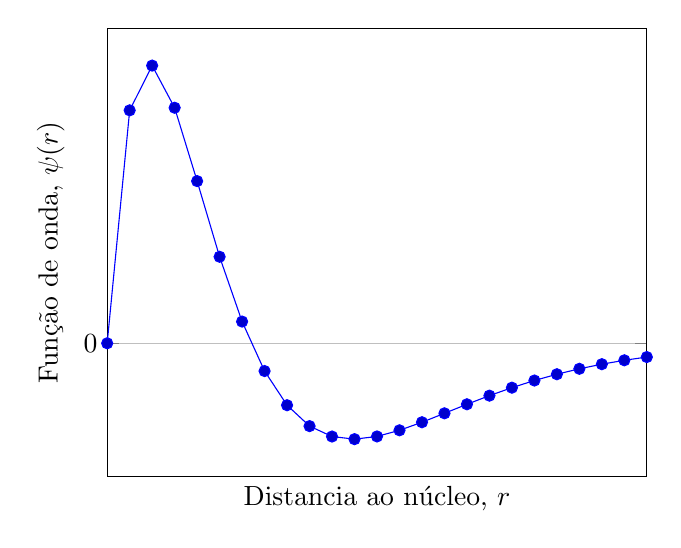
\begin{tikzpicture}
    \begin{axis}
    [
        grid=major,
        xlabel={Distancia ao núcleo, $r$},
        ylabel={Função de onda, $\psi(r)$},
        xmin=0,xmax=15,
        domain=0:15,
        ytick= {0},
        yticklabel={0},
        xtick = \empty,
    ]
    \addplot 
        { 100* 1/22 * x * (4-x) * e^(-x/2) };
    \end{axis}
\end{tikzpicture}